\section{Visibility and Shadows}


\subsection{Visibility}

We already encountered the \textbf{visibility problem}, some parts of some surfaces could be occluded. There are two possible solutions:
\begin{itemize}
	\item \textbf{Painter's Algorithm} - Render objects / polygons from furthest to nearest. This leads to problems when there are intersections or cyclic overlaps.
	\item \textbf{Z-Buffering} - Store depth to the nearest object for each pixel.
\end{itemize}

The Z-Buffering algorithm works as follows:
\begin{enumerate}
	\item Initialize all $z$ values to $\infty$.
	\item For each polygon: If $z$ value of a pixel for this polygon is smaller than the stored $z$ value, replace the stored $z$ value.
\end{enumerate}

The problem with this approach are that the resolution of the z-buffer is limited, we have to decide how many bits we need for the depth. If we think about how many bit to allocate, we also have to take into account that the depth resolution is not linear.


\subsection{Shadows}

Shadows are important as they can make an image immediately more realistic. There are different methods of creating shadows.

\subsubsection{Basic Shadows}

\textbf{Planar shadows} are the most basic approach, we simply draw a projection of the object on the ground. It is limited as it cannot create shadows on curved surfaces or other objects.
\begin{center}
	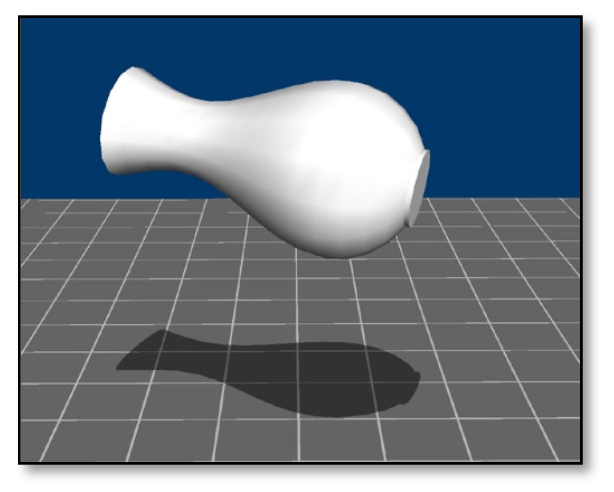
\includegraphics[width=0.5\linewidth]{planar_shadow.png}
\end{center}

\textbf{Projective texture shadows} uses texture mapping in a projective way. It works by creating a black and white image of the object from light. Then it uses this image as a projective texture. It is again limited as we need to define the obstacle and the receiver and it does not allow self-shadows.

\subsubsection{Shadow Maps}

The fundamental idea of shadow maps it to compute the depths from the light source. The depth from the light source gets save to a z-buffer (light source coordinates) we call this a \textbf{shadow map}. If we then render the scene from the camera position, we can transform each pixel $x_C$ from the camera coordinate system into the light coordinate system $x_L$. By comparing the depth of the corresponding value from the shadow map $d(x_L)$ and the projected point $z_L$, we can determine if a pixel gets illuminated or not. 
\begin{center}
	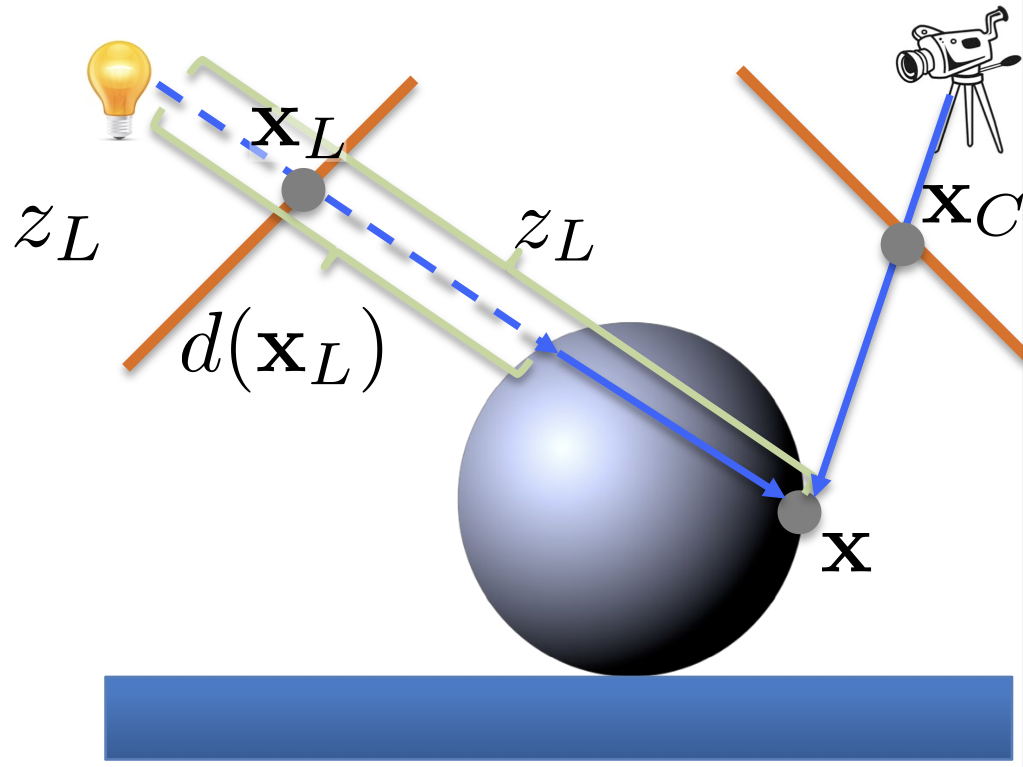
\includegraphics[width=0.8\linewidth]{shadow_map.png}
\end{center}

One of the main limitations of shadow maps is that there is a bias. Due to numerical errors it can happen that for a visible point $d(x_L) < z_L$. To avoid this we have to carefully select a bias to add to $d(x_L)$. \medskip

Another problem is the field of view. A point to shadow can be outside the field of view of the shadow map, due to the camera frustum. A solution to this would be to use a cubical shadow map or spot lights. \medskip

We might also occur aliasing, but we cannot filter depth. Instead we filter the result of the test by taking a weighted average of the comparisons.


\subsubsection{Shadow Volumes}

A third, more geometric, approach to rendering shadows are shadow volumes. For each light source we can explicitly represent the volume of space that is inside the shadow. If a polygon is inside the volume it is inside the shadow. To determine if a primitive is inside we apply the following algorithm:
\begin{enumerate}
	\item Shoot a ray from the camera
	\item Increment / decrement a counter each time the boundary of a shadow volume is intersected
	\item If the counter is 0, the primitive is not in the shadow
\end{enumerate}

This can be further optimized using silhouettes. Nevertheless this is very costly, as it introduces a lot of new geometry and we can only use the optimizations if objects are watertight.
